\documentclass[11pt,a4paper]{article}
\usepackage{fontspec}
\setmainfont{TeX Gyre Pagella}
\newfontfamily\headfont{Inter}[UprightFont=*-ExtraBold,BoldFont=*-ExtraBold,Extension=.otf,Path=/usr/share/fonts/opentype/inter/]
\usepackage[a4paper,margin=2.3cm]{geometry}
\usepackage{graphicx,booktabs,float,caption,array,xcolor}
\usepackage{xurl}
\usepackage[hidelinks]{hyperref}
\usepackage{titlesec}
\usepackage[round]{natbib}
\usepackage{setspace}
\setstretch{1.05}
\renewcommand{\topfraction}{0.9}
\renewcommand{\bottomfraction}{0.8}
\renewcommand{\textfraction}{0.1}
\renewcommand{\floatpagefraction}{0.75}
\setlength{\parindent}{0pt}
\setlength{\parskip}{0.55em}
\titleformat{\section}{\headfont\Large}{\thesection}{0.8em}{}
\titleformat{\subsection}{\headfont\large}{\thesubsection}{0.8em}{}
\captionsetup{font=small,labelfont=bf}
\urlstyle{same}
\hypersetup{pdftitle={Who's on the mountains?},pdfauthor={Tristan Hotham}}

\begin{document}
\begin{center}
{\Large\bfseries Who's on the mountains?\par}
\vspace{0.4em}
{\large The birthplaces of the people the world's mountains are named after\par}
\vspace{1.2em}
{\large Tristan Hotham\par}
\vspace{0.3em}
{\small Independent researcher\\
ORCID: 0000-0003-4931-9349\\
DOI: https://doi.org/10.5281/zenodo.24075305\par}
\vspace{0.8em}
2026
\end{center}

\begin{quote}
\small
\begin{center}\textbf{Abstract}\end{center}
Many of the world's mountains carry the names of people, often given by surveyors and explorers from far away. Using Wikidata's ``named after'' statements, I link 2,228 mountains, summits, hills, volcanoes and ranges to the 2,010 people they honour and to those people's birthplaces, after removing 49 wrong links and leaving unmapped 59 birthplaces that Wikidata gives only as a country, state or empire. In Europe 97.9\% of person-named mountains honour someone born in Europe; elsewhere the names are largely imported. 83.8\% of the person-named mountains of Australia and New Zealand honour someone born on another continent (78.9\% in Europe), as do 70.7\% in South America and 35.1\% in North America; outside Europe and Antarctica, 53.2\% honour someone born in Europe. Scientists (29.4\%) and royals, rulers and politicians (19.2\%) are the largest groups; women are 5.1\% of namings. Wikidata records a recent wave of renamings away from people's names, from Denali to Kuwohi. I describe the data, the errors found in it and its limits, and publish the linked table and an interactive map.

\textbf{Keywords:} toponymy; mountains; place names; commemoration; colonialism; surveying; Wikidata; open data; mapping
\end{quote}

\section{Introduction}
Mountains are among the most visible places to name, and among the most contested. In much of the world the names on the map are those of survey officers, patrons, monarchs and scientists, given in the eighteenth and nineteenth centuries by people from Europe to mountains that already had names in local languages. Mount Everest is the best known example: in 1856 Andrew Waugh of the Survey of India proposed the name of his predecessor as Surveyor General, George Everest, for Peak XV, and the Royal Geographical Society adopted it in 1865. Recent decades have seen a counter-movement, with official names restored or added in Indigenous languages, as with Denali in Alaska and Aoraki / Mount Cook in New Zealand.

This paper measures the pattern at a global scale with open data. Wikidata \citep{wikidata} records, for many mountains, the person they are named after (property P138) and, for many people, where they were born (P19). Joining the two gives each named mountain a line to a birthplace. A companion study did the same for the Moon and the planets; here the question is how far the names on Earth's own mountains travelled.

\section{Data}
A single query of Wikidata through QLever \citep{qlever} returned 11,175 rows: every item that is a mountain, summit, hill, volcano, range, sacred mountain or mountain pass and is named after a human, with coordinates, elevation and country, and the person's birthplace and its coordinates, date of birth, sex and occupations. Rows repeat for every type and occupation. After deduplication and the exclusions below there are 2,228 features and 2,241 feature and person pairs (``namings''; 13 features are named after two or more people), involving 2,010 people, 1,635 of them with a mappable birthplace. 769 features (34.5\%) are in Antarctica. Countries and continents are modern, from Natural Earth \citep{naturalearth}; anything south of 60$^\circ$S counts as Antarctica, and Svalbard is reported apart from mainland Norway.

\section{Methods}
\subsection{Exclusions and corrections}
81 mountain passes were removed, as gaps rather than mountains, with 16 features on the Moon and Mars (which Wikidata types as mountains) 6 undersea ridges and rises, and 3 features that are not mountains (two ravines and a road). Every naming whose feature name does not contain the namesake's name was read. 49 links were removed as wrong for the current name: the Gal\'apagos islands linked to the English nobles of their old English names, Lenin Peak linked to von Kaufman (its former name) and Avicenna (its Tajik name), Mount Clay to Ronald Reagan, former names such as Mount Stalin (Mount Peck since 1987), the Lenin Hills (now the Sparrow Hills) and Mount P\'etain (rescinded in 2022), and hills named after a saint by dedication through a church, chapel or shrine (Annaberg, Ai-Petri, Mont Saint-S\'ebastien), whose namesakes have legendary birthplaces. Birthplaces given only as a country, a state, a kingdom or an empire, often detectable from round coordinates at a region's centre, were left unmapped (59 people); 2 wrong birthplaces were corrected (Lyon Playfair, born at Chunar in India, not Haiti; and Mount Olga, now Kata Tjuta, named in 1872 after Queen Olga of W\"urttemberg, not the later Grand Duchess Olga born in 1895). All corrections are in \texttt{data/overrides.csv}.

\subsection{Elevations}
Wikidata elevations sometimes hold feet without saying so. Each value was compared with the highest point of the mountain's country; a value above it was read as feet if the converted value fits, and otherwise discarded. In Alaska only the named giants may exceed 4,000~m. A second check, against the highest points of US states and islands and against a coarse global elevation grid \citep{etopo5}, found eleven more values in feet (such as Mount Si and Mount Osceola) and one impossible value (Mount Rogers, given as higher than itself, the high point of Virginia), corrected by hand. 112 values were converted in all. Values in feet that are lower than any regional high point cannot be detected this way.

\subsection{Occupations and distance}
Occupations were grouped by keyword. Wikidata often gives a person several occupations, and a single priority list puts anyone also described as a politician, lawyer or activist (Kelvin, Wallace, Nansen, Amelia Earhart) among the rulers. Each person is therefore placed by tiers: titles of rule (monarch, consort, president, governor, revolutionary); then specific professions, in the order military and naval officers, surveyors and cartographers, explorers, mountaineers and aviators, scientists (including physicians), saints and clergy; then politics without a title (politician, diplomat, lawyer, judge); then writers, artists and business people; then generic labels (military personnel, engineer, university teacher, writer). The first tier with a match decides. Other rules move the shares by several points, but not the order of the main groups. Distances are great circles between the feature and the birthplace.

\section{Results}
\subsection{An imported geography}
Figure~\ref{fig:world} maps every naming. Within Europe names are local: 97.9\% of person-named European mountains honour someone born in Europe and 17.2\% someone born in the same country. Elsewhere they are not (Figure~\ref{fig:cont}, Table~\ref{tab:cont}). In Oceania 84.3\% honour someone born on another continent; in South America 70.7\%; in North America 35.1\%, where 34.2\% honour people born in Europe. Over all mountains outside Europe and Antarctica, 53.2\% of namings honour someone born in Europe, and the median line from mountain to birthplace is 3,289~km long. By country (Figure~\ref{fig:countries}), 87.5\% of New Zealand's person-named mountains and 83.8\% of Australia's honour people born abroad, mostly in the United Kingdom, against 29.0\% in the United States. Svalbard (73.0\% foreign-born, mostly Swedish, German and British) reflects its history of international scientific exploration. All 621 located Antarctic namings honour people born elsewhere, 73.3\% in Europe.

\begin{figure}[tbp]\centering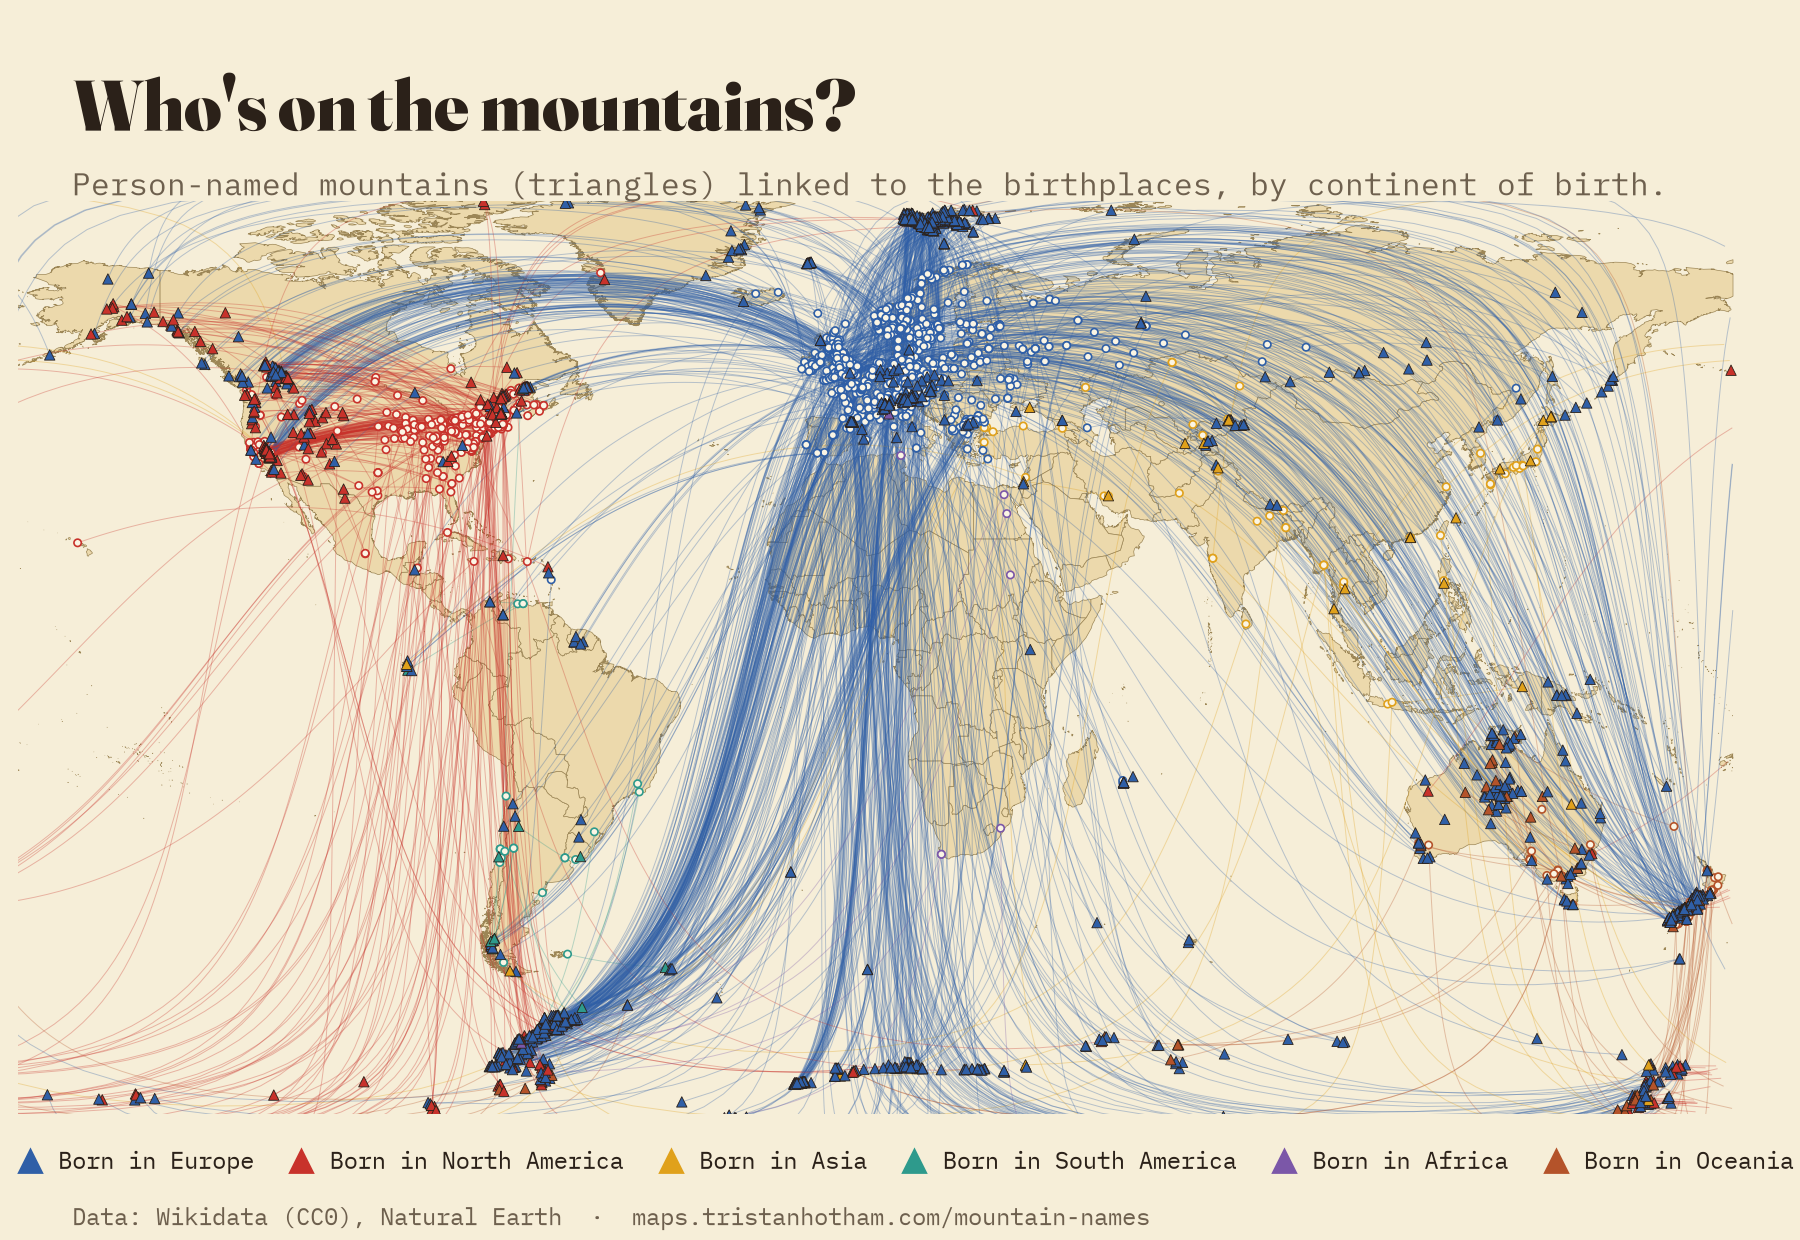
\includegraphics[width=\textwidth]{f_world.png}
\caption{Mountains named after a person, with great-circle lines to the person's birthplace, coloured by continent of birth.}\label{fig:world}\end{figure}
\begin{figure}[tbp]\centering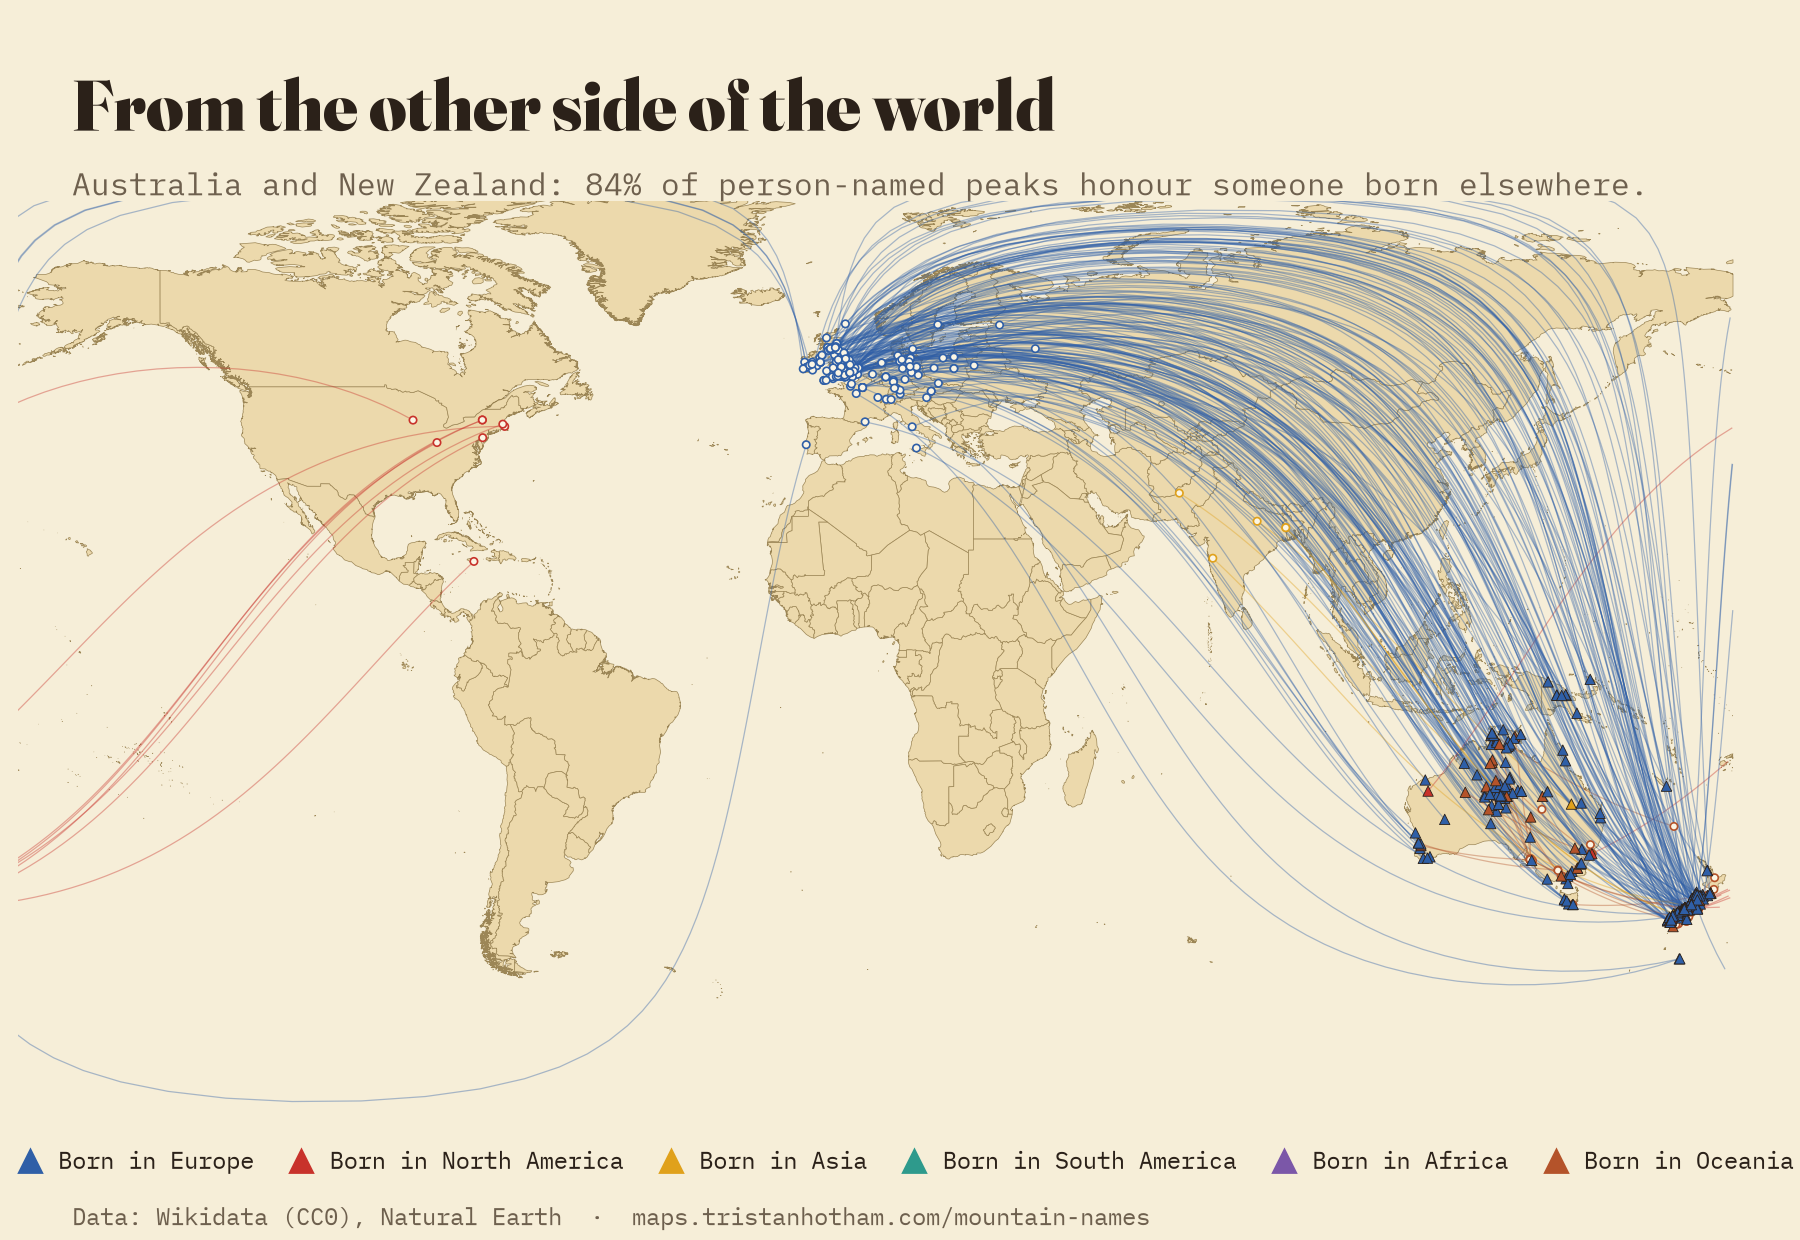
\includegraphics[width=\textwidth]{f_oceania.png}
\caption{The person-named mountains of Australia and New Zealand and their namesakes' birthplaces.}\label{fig:oceania}\end{figure}
\begin{figure}[tbp]\centering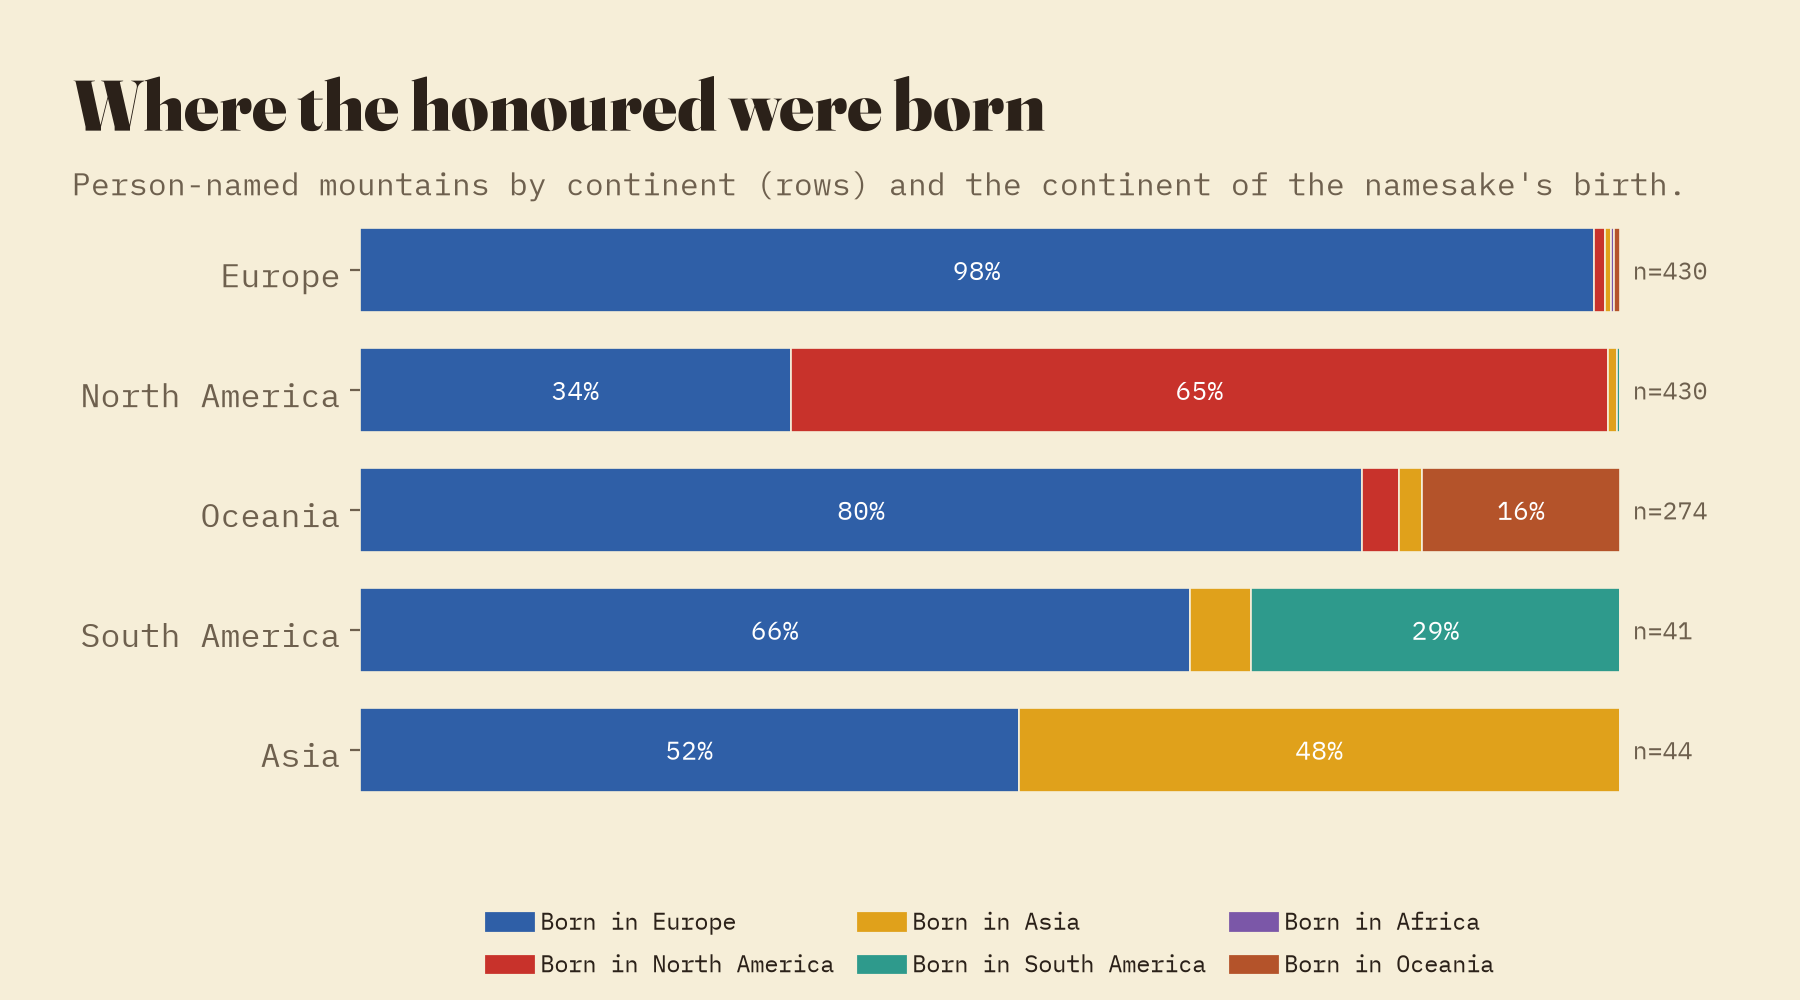
\includegraphics[width=0.9\textwidth]{f_continents.png}
\caption{Continent of birth of namesakes, by continent of the mountain.}\label{fig:cont}\end{figure}

\begin{table}[tbp]\centering\small\caption{Located namings by continent of the mountain: share honouring someone born in Europe, on another continent, and in the same modern country.}\label{tab:cont}\begin{tabular}{lrrrr}\toprule Continent & Namings & Born in Europe (\%) & Other continent (\%) & Same country (\%)\\\midrule
Europe & 430 & 97.9 & 2.1 & 17.2\\
North America & 430 & 34.2 & 35.1 & 59.8\\
Oceania & 274 & 79.6 & 84.3 & 13.5\\
South America & 41 & 65.8 & 70.7 & 14.6\\
Asia & 44 & 52.3 & 52.3 & 40.9\\
Antarctica & 621 & 73.3 & 100.0 & \\
\bottomrule\end{tabular}\end{table}

\begin{figure}[tbp]\centering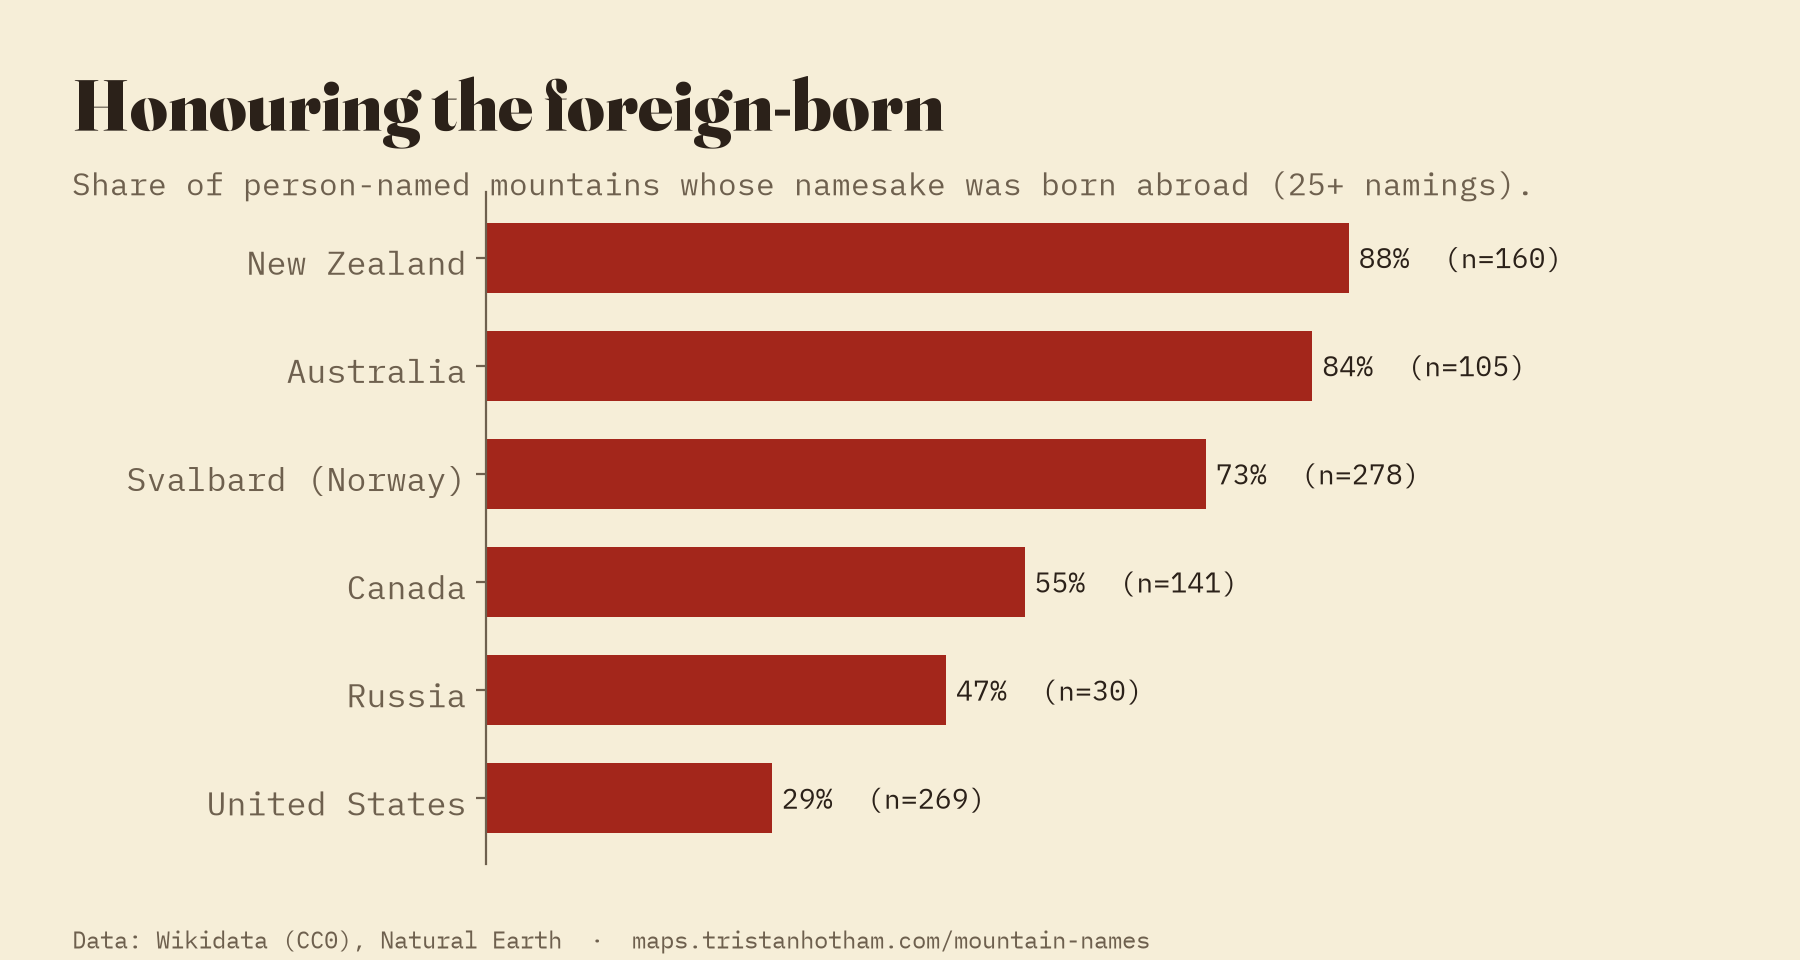
\includegraphics[width=0.9\textwidth]{f_countries.png}
\caption{Share of person-named mountains honouring someone born in another country, for countries with 25 or more located namings.}\label{fig:countries}\end{figure}

\subsection{Who is honoured}
Scientists are the largest group (29.4\% of namings with an occupation), then royals, rulers and politicians (19.2\%, the largest group in North America and Oceania), explorers, mountaineers and aviators (17.3\%), military and naval officers (11.8\%) and surveyors, geographers and cartographers (10.9\%) (Figure~\ref{fig:occ}). Survey networks honoured their own: the California Geological Survey of the 1860s named High Sierra peaks after its leader Josiah Whitney, its members and its scientific mentors. The most honoured person is the botanist Ferdinand von Mueller (6 features). The median namesake was born in 1853; 65.7\% were born in the nineteenth century.

\begin{figure}[tbp]\centering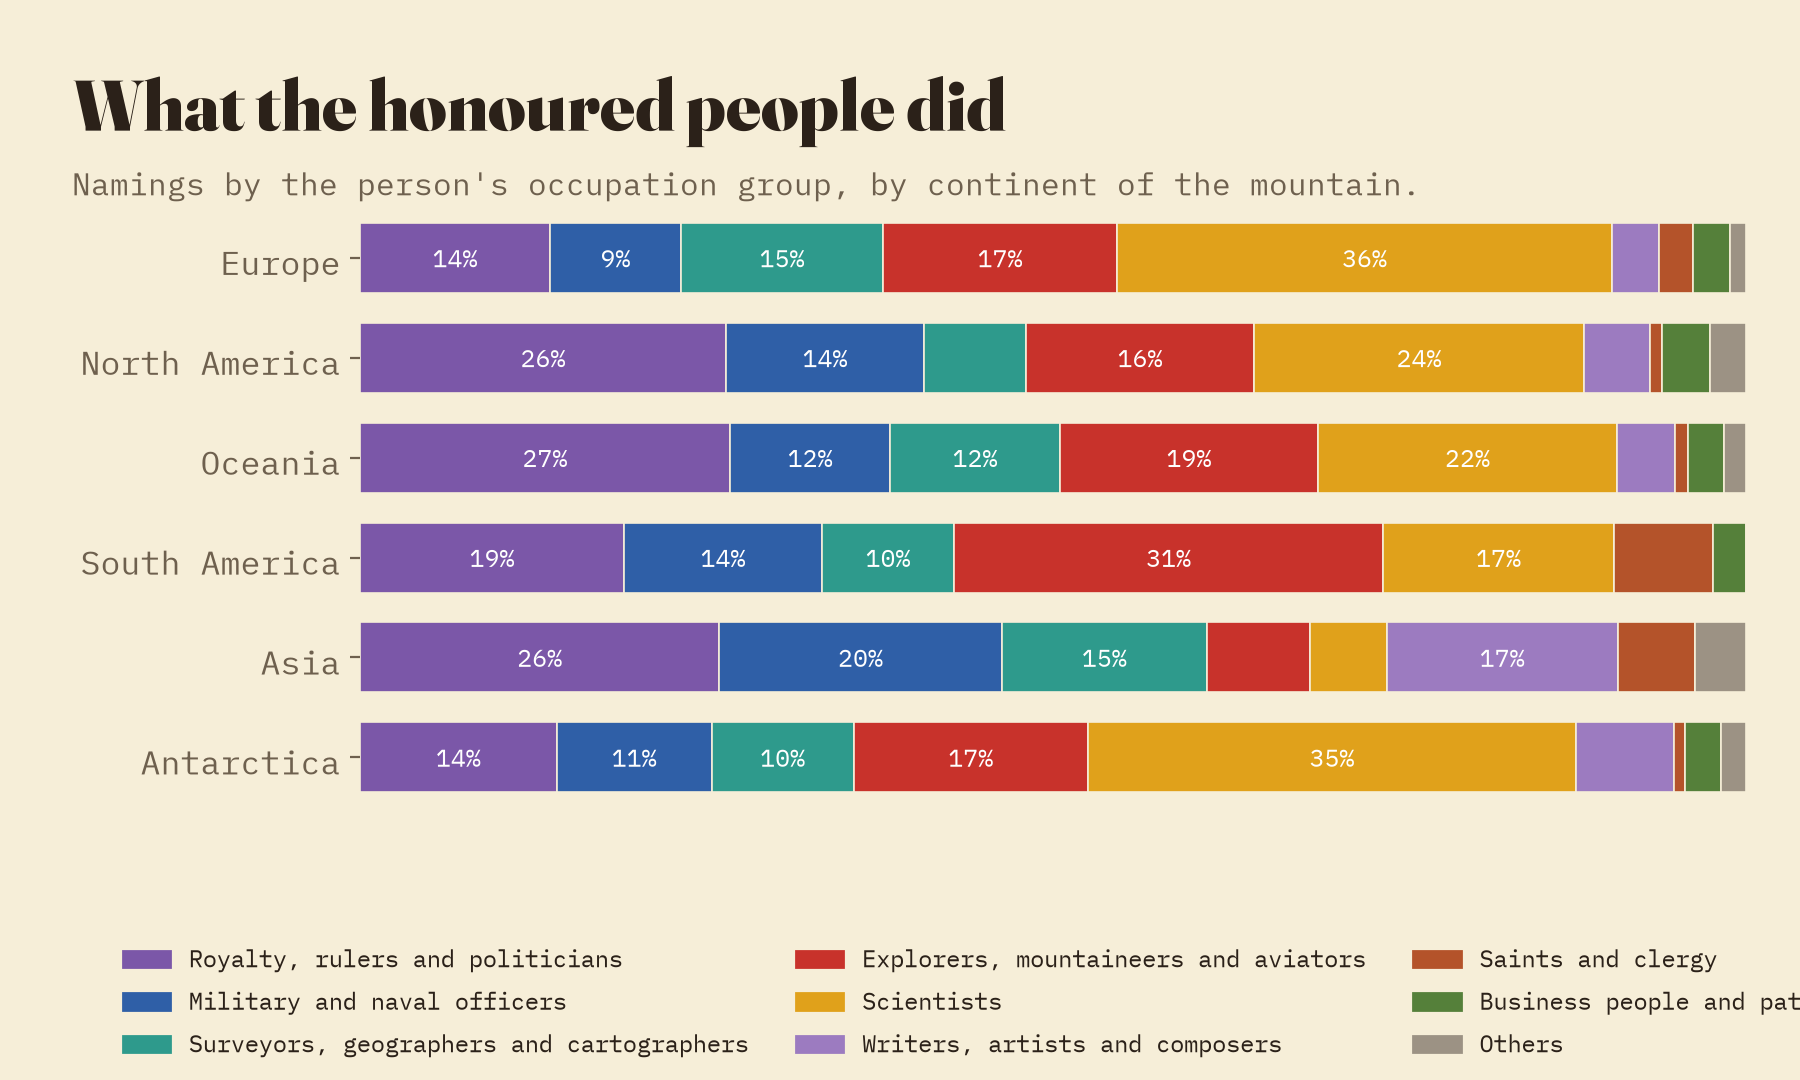
\includegraphics[width=0.9\textwidth]{f_occupations.png}
\caption{Occupation groups of namesakes, by continent of the mountain.}\label{fig:occ}\end{figure}

\subsection{Women}
Of 2,224 namings whose person has a recorded sex, 113 (5.1\%) honour a woman; 30.1\% of those are royals or politicians, against 17.1\% of the men. The share is 11.5\% among people born since 1900 and 3.9\% among those born earlier.

\subsection{The highest}
Table~\ref{tab:tall} and Figure~\ref{fig:tall} list the highest person-named mountains: Everest, Ismoil Somoni Peak and Lenin Peak, then several Pamir peaks named in the Soviet period after revolutionaries and scientists.

\begin{table}[tbp]\centering\footnotesize\caption{The fifteen highest person-named mountains in Wikidata (* converted from feet).}\label{tab:tall}\begin{tabular}{lrlll}\toprule Mountain & m & Named after & Country & Born in\\\midrule
Mount Everest & 8,849 & George Everest & Nepal and China & United Kingdom\\
Ismoil Somoni Peak & 7,495 & Ismail Samani & Tajikistan & Uzbekistan\\
Lenin Peak & 7,134 & Vladimir Lenin & Tajikistan & Russia\\
Dzerzhinsky Peak & 6,717 & Felix Dzerzhinsky & Tajikistan & Belarus\\
Tipas & 6,658 & Walther Penck & Argentina & Austria\\
Parrota & 6,277 & Friedrich Parrot & Tajikistan & Germany\\
Przhevalsky peak & 6,276 & Nikolay Przhevalsky & China & not mapped\\
Cerro General Belgrano & 6,250 & Manuel Belgrano & Argentina & Argentina\\
Denali (Mount McKinley) & 6,190 & William McKinley & United States & United States\\
Churchill Peaks & 6,167* & Winston Churchill & United States & United Kingdom\\
Euler Peak & 6,022 & Leonhard Euler & Kyrgyzstan & Switzerland\\
Schlagintweit Peak & 5,971 & Adolf von Schlagintweit & Pakistan & Germany\\
Mount Logan & 5,959 & William Edmond Logan & Canada & Canada\\
Semyonov peak & 5,816 & Pyotr Semyonov-Tyan-Shansky & Kazakhstan & Russia\\
Pico Simón Bolívar & 5,775 & Simón Bolívar & Colombia & Venezuela\\
\bottomrule\end{tabular}\end{table}

\begin{figure}[tbp]\centering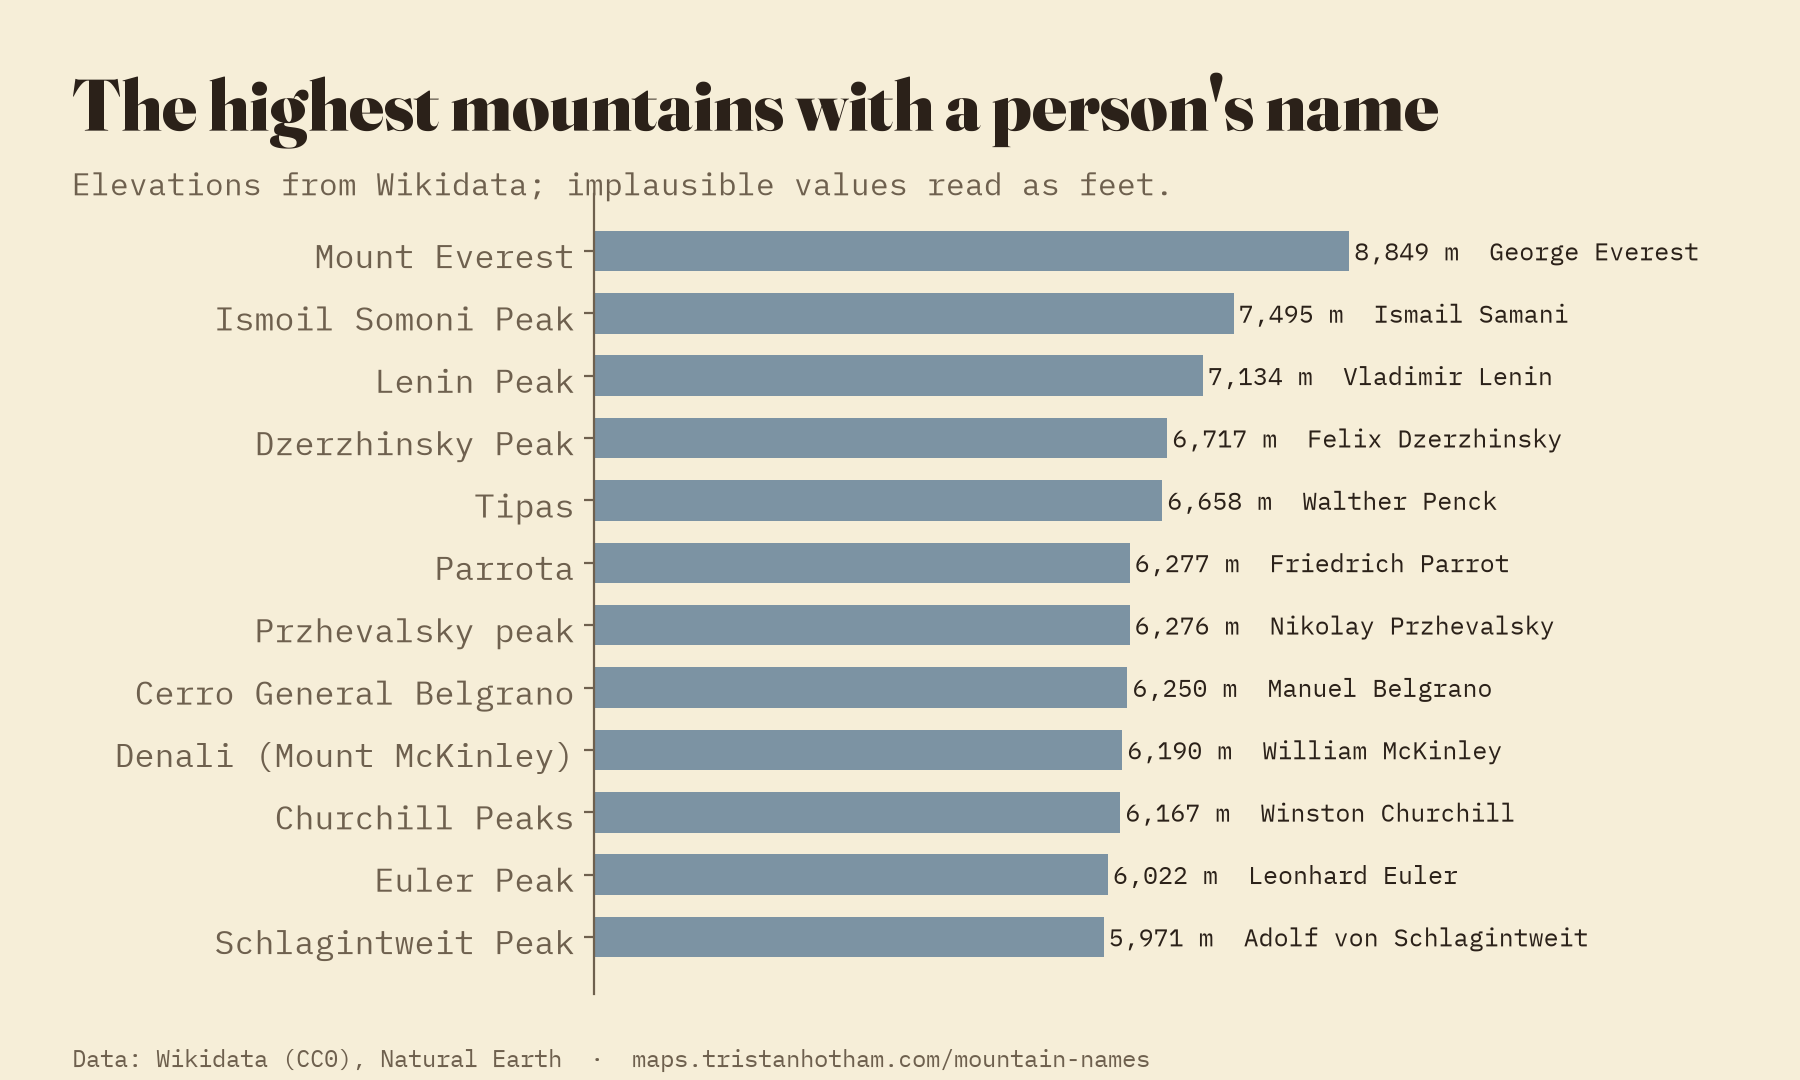
\includegraphics[width=0.9\textwidth]{f_tallest.png}
\caption{The highest mountains named after a person in Wikidata.}\label{fig:tall}\end{figure}

\subsection{Renamings}
Wikidata's dated official names record renamings away from people (Table~\ref{tab:ren}): Mount McKinley to Denali (2015; Mount McKinley again as the US federal name by presidential order from 2025, while the State of Alaska, which adopted Denali in 1975, keeps it), Harney Peak to Black Elk Peak (2016), Jeff Davis Peak to Doso Doyabi (2019), Mount Evans to Mount Blue Sky (2023) and Clingmans Dome to Kuwohi (2024). Others appear as ``named after'' links that survive from a former name (King Leopold Ranges, Mount Stalin, Lenin Hills). Renamings towards people also occur (Dzyarzhynskaya Hara, 1958). Nine features carry dual names, such as Aoraki / Mount Cook and Kunanyi / Mount Wellington. In 2022 the US Board on Geographic Names replaced a slur for Native American women in the names of nearly 650 features; Wikidata records 96 of them that are hills, peaks or mountains.

\begin{table}[tbp]\centering\small\caption{Renamed mountains recorded in Wikidata.}\label{tab:ren}\begin{tabular}{p{4.2cm}p{3.6cm}p{3.6cm}r}\toprule Now & Before & Honoured before & Year\\\midrule
Denali & Mount McKinley & William McKinley & 2015\\
Black Elk Peak & Harney Peak & William S. Harney & 2016\\
Mount Blue Sky & Mount Evans & John Evans & 2023\\
Doso Doyabi & Jeff Davis Peak & Jefferson Davis & 2019\\
Kuwohi & Clingmans Dome & Thomas Lanier Clingman & 2024\\
Unnamed peak (formerly Mount Pétain) & Mount Pétain & Philippe Pétain & 2022\\
Wunaamin-Miliwundi Ranges & King Leopold Ranges & Leopold II of Belgium & 2020\\
Mount Peck & Mount Stalin & Joseph Stalin & 1987\\
Sparrow Hills & Lenin Hills & Vladimir Lenin & \\
Lenin Peak & Kaufmann Peak & Konstantin von Kaufman & \\
Dzyarzhynskaya Hara & Skirmantava &  & 1958\\
Pik Bilibina & Snezhnaya &  & 2003\\
\bottomrule\end{tabular}\end{table}

\section{Limitations}
Wikidata is not a complete list of named mountains: its coverage follows the work of its editors and imported gazetteers, and is dense for the Sierra Nevada, Svalbard, New Zealand and Antarctica and thin for much of Asia, Africa and South America, where few mountains in the extract are named after people. ``Named after'' statements can refer to a former name; I removed those I found. Modern borders are applied to historical birthplaces. Occupations are coarse, depend on Wikidata's lists and on the grouping rule. Sex is as Wikidata records it. Elevations are as Wikidata gives them, with the conversions described.

\section{Conclusion}
The names on the world's mountains are, outside Europe, overwhelmingly the names of Europeans and of the settler states' own officials, scientists and rulers, often given from the other side of the globe. The open data make the pattern measurable and show the slow work of renaming that is now under way.

\section*{Data and code availability}
The interactive map is at \url{https://maps.tristanhotham.com/mountain-names/}. Data and code are at \url{https://github.com/Tristan-Hotham/mountain-names} and archived with this paper at https://doi.org/10.5281/zenodo.24075305. Derived data and text are released under CC BY 4.0 (Wikidata is CC0); code under the MIT licence.

\section*{AI statement}
I wrote the text, with drafting and editing assistance from Claude (Anthropic), which also helped prepare the analysis code. I reviewed and checked all text and results.

\begin{thebibliography}{9}
\bibitem[Bast and Buchhold(2017)]{qlever} Bast, H. and Buchhold, B. (2017) QLever: a query engine for efficient SPARQL+Text search. In \textit{Proceedings of the 2017 ACM Conference on Information and Knowledge Management (CIKM)}, 647 to 656.
\bibitem[National Geophysical Data Center(1988)]{etopo5} National Geophysical Data Center (1988) \textit{ETOPO5: Five-minute gridded elevations and bathymetry for the world}. Boulder: NOAA.
\bibitem[Natural Earth(2026)]{naturalearth} Natural Earth (2026) Admin 0 countries 1:10m and populated places. Public domain. \url{https://www.naturalearthdata.com/}
\bibitem[Vrande\v{c}i\'c and Kr\"otzsch(2014)]{wikidata} Vrande\v{c}i\'c, D. and Kr\"otzsch, M. (2014) Wikidata: a free collaborative knowledgebase. \textit{Communications of the ACM} 57(10), 78 to 85.
\end{thebibliography}
\end{document}
